\documentclass[a4paper]{article}

\linespread{1.1}
\usepackage[utf8]{inputenc} 
\usepackage[T1]{fontenc}
\usepackage[francais]{babel}
\usepackage{amsmath}
\usepackage{amsfonts}
\usepackage{amssymb}
\usepackage{graphicx}
\usepackage{lmodern}
\usepackage{microtype}
\usepackage{hyperref}
\usepackage[margin=1.8cm]{geometry}
\usepackage{pgf,tikz}
\usepackage{mathrsfs}
\usetikzlibrary{arrows}


% Structure

\newcounter{c}
\newcounter{d}
\newcounter{r}
\newcounter{e}

\newcommand{\defi}{\subparagraph{Definition \arabic{c}.\arabic{d} :}\stepcounter{d}}
\newcommand{\prop}{\subparagraph{Proposition \arabic{c}.\arabic{r} :}\stepcounter{r}}
\newcommand{\thm}{\subparagraph{Theorem \arabic{c}.\arabic{r} :}\stepcounter{r}}
\newcommand{\demo}{\subparagraph{Proof}}
\newcommand{\cor}{\subparagraph{Corollary \arabic{c}.\arabic{r} :}\stepcounter{r}}
\newcommand{\lem}{\subparagraph{Lemma \arabic{c}.\arabic{r} :}\stepcounter{r}}
\newcommand{\rem}{\subparagraph{Remark :}}
\newcommand{\chapitre}[1]{\stepcounter{c}\setcounter{e}{0}\setcounter{d}{0}\setcounter{r}{0}\noindent\textbf{\Large#1}\\}
\newcommand{\eq}[1]{\stepcounter{e}\begin{equation}#1\tag{\arabic{c}.\arabic{e}}\end{equation}}

% Notations

\newcommand{\Q}{\mathbb{Q}}
\newcommand{\Z}{\mathbb{Z}}
\newcommand{\N}{\mathbb{N}}
\newcommand{\R}{\mathbb{R}}
\newcommand{\C}{\mathbb{C}}
\newcommand{\E}[1]{\mathbb E\left(#1\right)}
\newcommand{\sph}{\mathbb{S}}
\newcommand{\p}{{\cal{P}}}
\newcommand{\fsp}{{\cal{F}}}
\newcommand*{\qed}{\hfill\ensuremath{\square}}
\newcommand{\x}{\mathbf x}
\newcommand{\y}{\mathbf y}
\newcommand{\e}{\mathbf e}
\newcommand{\scal}[2]{\langle#1,#2\rangle}
\newcommand{\trans}{^\text{T}\!}
\newcommand{\dt}{\frac d{dt}}

\newcommand{\dpart}[2]{\displaystyle\frac{\partial#1}{\partial #2}}

\newcommand{\nor}[2]{{\cal N}(#1,#2)}
\newcommand{\mat}[2]{{\cal M}_{#1\times#2}(\R)}

\newcommand{\X}{\mathbf X}

\renewcommand{\leq}{\leqslant}
\renewcommand{\geq}{\geqslant}

\newcommand{\vertiii}[1]{{\left\vert\kern-0.25ex\left\vert\kern-0.25ex\left\vert #1\right\vert\kern-0.25ex\right\vert\kern-0.25ex\right\vert}}


\begin{document}\stepcounter{c}

\paragraph{\arabic{c} - Model reduction : 3D to 1D}~


Consider a compliant straight vessel whose axis coincides with the $x-$axis of a castesian coordinate system. We denote $V_t$ the domain of interest at time $t$. The following discussion is based on Reynolds' transport therorem :

\thm If $f(\mathbf x,t)$ is continuous, then :
\eq{\dt\int_{V_t}fdV=\int_{V_t}\frac{\partial f}{\partial t}+\int_{\partial V_t}f\mathbf u_b\cdot\mathbf ndS}

where $\mathbf n$ denotes the normal vector at the current point on the wall, and $\mathbf u_b$ denotes the boundary displacement. Let us write $\sigma_1$ and $\sigma_2$ for the input ($x=x_1$) and output ($x=x_2$) boundaries respectively. We suppose :
\begin{itemize}
\item $\mathbf u_b\cdot\mathbf n=0$ on $\sigma_1$ and $\sigma_2$,
\item $\mathbf u_b=\mathbf u_w$ on $\partial V_{t,w}$ ("w" for "wall").
\end{itemize}

We want to derive a 1D representation of this vessel. If $A(x,t)$ is the area of section $\sigma(x,t)$ of abscissa $x$ at time $t$, we define the surfacic mean of $f$ :

\eq{\overline{f}(x,t)=\frac1{A(x,t)}\int_\sigma fdS}

\noindent It follows :

\eq{\int_{V_t}fdV=\int_{x_1}^{x_2}\int_\sigma fdSdx=\int_{x_1}^{x_2}A(x,t)\overline{f}(x,t)dx}

\noindent If $x_1$ and $x_2$ are constant with respect to time, we have :

\eq{\dt\int_{V_t}fdV=\int_{x_1}^{x_2}\frac{\partial}{\partial t}\left(A(x,t)\overline{f}(x,t)\right)dx}

\noindent Wall displacement with respect to fluid is given by :

$$\mathbf w=\mathbf u_w-\mathbf u$$

\noindent We get :

\eq{\int_{\partial V_t}f\mathbf u_v\cdot\mathbf n dS=\int_{\partial V_{t,w}}f\mathbf u_w\cdot\mathbf n dS=\int_{\partial V_{t,w}}f\mathbf w\cdot\mathbf n dS+\int_{\partial V_{t,w}}f\mathbf u\cdot\mathbf n dS}

\noindent Writing $\mathbf u=(u_x,u_y,u_z)$ and since $\mathbf u\cdot\mathbf n\leq0$ on $\sigma_1$ and $\geq0$ on $\sigma_2$ :

\eq{\int_{\partial V_{t,w}}f\mathbf u\cdot\mathbf ndS=\int_{\partial V_t}f\mathbf u\cdot\mathbf ndS+\int_{\sigma_1}fu_xdS-\int_{\sigma_2}fu_xdS}

\noindent Applying Gauss' divergence theorem :

$$\int_{\partial V_t}f\mathbf u\cdot\mathbf ndS=\int_{V_t}\nabla\cdot(f\mathbf u)dV$$

\noindent yields :

\eq{\int_{\partial V_{t,w}}f\mathbf u_w\cdot\mathbf ndS=\int_{\partial V_{t,w}}f\mathbf w\cdot\mathbf ndS+\int_{V_t}\nabla\cdot(f\mathbf u)dV+\int_{\sigma_1}fu_xdS-\int_{\sigma_2}fu_xdS}

\noindent but :

\eq{\int_{\sigma_1}fu_xdS-\int_{\sigma_2}fu_xdS=\left(A(x_1,t)-A(x_2,t)\right)\overline{(fu_x)}=-\int_{x_1}^{x_2}\frac{\partial}{\partial x}A(x,t)\overline{(fu_x)}dx}

\noindent so :

\eq{\int_{\partial V_{t,w}}f\mathbf u_w\cdot\mathbf ndS=\int_{\partial V_{t,w}}f\mathbf w\cdot\mathbf ndS+\int_{V_t}\nabla\cdot(f\mathbf u)dV-\int_{x_1}^{x_2}\frac{\partial}{\partial x}A(x,t)\overline{(fu_x)}dx}

\noindent Starting again from equation (1.1) and using equations (1.3), (1.4) and (1.9), we find :

\eq{\int_{x_1}^{x_2}\frac{\partial}{\partial t}\left(A\overline{f}\right)dx=\int_{x_1}^{x_2}\left(\int_\sigma\left(\frac{\partial f}{\partial t}+\nabla\cdot(f\mathbf u)\right)dS+\int_{\partial \sigma}\mathbf w\cdot\mathbf ndL-\frac{\partial}{\partial x}A(\overline fu_x)\right)dx}

\noindent and since it works for every choice of $x_1$ and $x_2$, we may write :

\eq{\frac{\partial}{\partial t}(A\overline f)=\int_\sigma\left(\frac{\partial f}{\partial t}+\nabla\cdot(f\mathbf u)\right)dS+\int_{\partial\sigma}\mathbf w\cdot\mathbf ndL-\frac{\partial}{\partial x}A(\overline fu_x)}

\noindent Taking $f\equiv1$ gives the mass conservation equation :

\eq{\frac{\partial A}{\partial t}-\frac{\partial(Au_x)}{\partial x}=\int_\sigma\nabla\cdot\mathbf udS+\int_{\partial\sigma}\mathbf w\cdot\mathbf ndL}

\noindent with $\nabla\cdot\mathbf u=0$ if the fluid is incompressible.

\bigskip

\noindent Taking $f=u_x$ yields the moment equilibrium equation :

\eq{\frac{\partial}{\partial t}(A\overline{u_x})+\frac{\partial}{\partial x}(A\overline{u^2_x})=\int_\sigma\left(\frac{\partial u_x}{\partial t}+\nabla\cdot(u_x\mathbf u)\right)dS+\int_{\partial S}u_x\mathbf w\cdot\mathbf ndL}

\noindent yielding in incompressible case :

\eq{\frac{\partial}{\partial t}(A\overline{u_x})+\frac{\partial}{\partial x}(A\overline{u^2_x})=\int_\sigma\left(\frac{\partial u_x}{\partial t}+\mathbf u\cdot\nabla u_x\right)dS+\int_{\partial S}u_x\mathbf w\cdot\mathbf ndL}

\defi The \emph{material derivative} is the differential operator :

$$\mathbf D=\frac{\partial}{\partial t}+\mathbf u\cdot\nabla$$

\noindent One can show that :

\eq{\int_\sigma\mathbf Du_xdS=\int_\sigma\left(f_x^b+\frac1\rho\left(-\frac{\partial p}{\partial x}+d_x\right)\right)dS}

\noindent where $f^b$ represents the body force per unit volume, $\rho$ the fluid density and $\mathbf d=\nabla\cdot\mathbf D$.


It follows :

\eq{\frac{\partial}{\partial t}(A\overline{u_x})+\frac{\partial}{\partial x}(A\overline{u^2_x})=\int_\sigma\left(f_x^b+\frac1\rho\left(-\frac{\partial p}{\partial x}+d_x\right)\right)dS+\int_{\partial\sigma}u_x\mathbf w\cdot\mathbf ndL}

\noindent yielding :

\eq{\frac\partial{\partial t}(A\overline{u_x})+\frac\partial{\partial x}(A\overline{u_x^2})=\frac A\rho\left(\rho\overline{f_x^b}-\frac{\partial\overline p}{\partial x}+\overline{d_x}\right)+\int_{\partial\sigma}u_x\mathbf w\cdot\mathbf ndL}

\noindent Furthermore, we consider :
\begin{itemize}
\item $\overline{u_x^2}=\alpha\overline{u_x}^2$, where $\alpha$ is the Coriolis coefficient determining the velocity profile,
\item $\displaystyle \frac A\rho\overline{d_x}=-K_Ru_x$ where $K_R$ is the viscous resistance coefficient.
\end{itemize}

\noindent We thus find the momentum conservation equation :

\eq{\frac\partial{\partial t}(A\overline{u_x})+\frac\partial{\partial x}(\alpha A\overline{u_x}^2)=A\overline{f_x^b}-\frac A\rho\left(\frac{\partial\overline p}{\partial x}\right)-K_R\overline{u_x}+\int_{\partial\sigma}u_x\mathbf w\cdot\mathbf ndL}

\rem Thsi last equation (1.18) is the momentum equilibrium equation, where :
\begin{itemize}
\item $\mathbf w\cdot\mathbf n=0$ if the wall is impermeable,
\item $f^b_x\simeq0$ if body forces are neglectible.
\end{itemize}



\newpage
\stepcounter{c}
\setcounter{d}{0}
\setcounter{e}{0}
\paragraph{\arabic{c} - Model reduction : 1D to 0D}~


\defi Let $Q(x,t)$ be the flow through a cross section $\sigma(x,t)$ :

$$Q(x,t)=A(x,t)\overline{u_x}=\int_{\sigma(x,t)}u_xdS$$

\noindent Mass and momentum conservation equations (1.12) and (1.18) become :

\eq{\dpart At+\dpart Qx=0}
\eq{\dpart Qt+\dpart{}x\left(\alpha\frac{Q^2}A\right)+\frac A\rho\left(\dpart pt\right)+K_R\frac QA=0}

\noindent where $p$ denotes $\overline p$ for the sake of simplicity.

\defi If $l=|x_2-x_1|$, we define the volumic mean flow :

$$\hat Q(t)=\frac\rho l\int_{\Omega_t} u_x(x,t)dV=\frac\rho l\int_{x_1}^{x_2}\left(\int_{\sigma(x,t)} u_x(x,t)dS\right)dx=\frac\rho l\int_{x_1}^{x_2}Q(x,t)dx$$

\noindent Same thing with pressure and cross-sectional area :
$$\hat p=\frac1l\int_{x_1}^{x_2}pdx~~\text{ and }~~\hat A=\frac1l\int_{x_1}^{x_2}Adx$$

We are now able to reduce our 1D model to a 0D one by integrating along the $x$-axis between $x_1$ and $x_2$ the two equations (2.1) and (2.2), thanks to the two following assumptions :

\begin{itemize}
\item the convective term is neglectible : $\dpart{}x\left(\alpha\frac {Q^2}A\right)\simeq 0$,
\item $\left|\dpart Ax\right|<<\left|\dpart px\right|,\left|\dpart Qx\right|$.
\end{itemize}

\noindent We will thus replace $A$ in the equations by its value at rest $A_0$.

\bigskip

\noindent Using obvious notations, the equations become :

\eq{l\frac{d\hat A}{dt}+Q_2-Q_1=0}
\eq{\frac{\rho l}{A_0}\frac{d\hat Q}{dt}+\frac{\rho K_Rl}{A_0^2}\hat Q+P_2-P_1=0}

\noindent We now have to close this system with a wall mechanics law :

\eq{\int_{x_1}^{x_2}\dpart ptdx=\int_{x_1}^{x_2}\frac\beta{2\sqrt A}\dpart Atdx}

\noindent yielding, thanks to our assumptions :

$$l\frac{d\hat p}{dt}=\frac{l\beta}{2\sqrt{A_0}}\frac{d\hat A}{dt}$$

\noindent which we may write :

$$\frac{d\hat A}{dt}=k_1\frac{d\hat p}{dt}$$

\noindent for convenience, where $k_1=\frac{2\sqrt{A_0}}{\beta}$. Equation (2.3) becomes :

\eq{k_1l\frac{d\hat p}{dt}+Q_2-Q_1=0}

\defi We define the \emph{resistance}, \emph{inductance} and \emph{capacitance} coefficients, respectively :

$$R=\frac{\rho K_R l}{A_0^2}~~~~L=\frac{\rho l}{A_0}~~~~C=k_1l$$

\subparagraph{Example :} For a Poiseuille flow, if $r_0$ is the lumen radius and $h_0$ the wall thickness at rest, we have :

$$R=\frac{8\rho\nu l}{\pi r_0^4}~~~~L=\frac{\rho l}{\pi r_0^2}~~~~C=\frac{3\pi r_0^3l}{2Eh_0}$$

Our lumped parameter model becomes :

\eq{\left\{\begin{array}{l}\displaystyle C\frac{d\hat p}{dt}+Q_2-Q_1=0\\\displaystyle L\frac{d\hat Q}{dt}+R\hat Q+P_2-P_1=0\end{array}\right.}

\bigskip

Thsi discussion allows us to approximate compliant pipes with electric networks. Typically, a short pipe is approximated by a $\mathcal L$-network or a $\mathcal L$-inverted network. The model choice depends on the data available.

\begin{center}
\begin{tikzpicture}
\draw[->] (0,0)--(0.4,0);
\draw[->] (3.6,0)--(4,0);
\draw[->] (0.4,-0.9)--(0.4,-0.1);
\draw[->] (3.6,-0.9)--(3.6,-0.1);

\draw (0.5,0)--(1.5,0) (2,0)--(2.5,0) (3.1,0)--(3.5,0) (1,0)--(1,-0.5) (1,-0.6)--(1,-1) (0.5,-1)--(3.5,-1);

\draw (0.8,-0.5)--(1.2,-0.5) (0.8,-0.6)--(1.2,-0.6);
\draw (1.5,0)--(1.55,0.1)--(1.6,-0.1)--(1.65,0.1)--(1.7,-0.1)--(1.75,0.1)--(1.8,0)--(2,0);
\draw (2.5,0) to [out=90,in=90] (2.65,0) to [out=90,in=90] (2.8,0) to [out=90,in=90] (2.95,0) to [out=90,in=90] (3.1,0);

\draw (-0.3,0) node {$Q_1$} (4.3,0) node {$Q_2$} (0.1,-0.5) node {$P_1$} (3.9,-0.5) node {$P_2$} (1.65,0.3) node {$R$} (2.8,0.3) node {$L$} (1.4,-0.5) node {$C$};
\end{tikzpicture}


~


$\mathcal L-network$
\end{center}




\stepcounter{c}
\paragraph{\arabic{c} - Lumped model : a testcase}~


We consider a lumped 0D RCR model for a tubular elastic blood vessel : a resistor $R_1$ at the flow input $q(t)$ connected to a grounded (output) resistor $R_2$ and a grounded capacitor $C$. The total pressure (input-to-ground voltage) is denoted by $p$, and $\pi$ the nodal pressure (node-to-ground voltage).


\begin{center}
\begin{tikzpicture}
\draw (-1.7,0)--(-1.3,0);
\draw (1.3,0)--(1.7,0);
\draw (0,-1)--(0,-1.4);
\draw (-0.7,0)--(0.7,0);
\draw (0,0)--(0,-0.8);

% resistors
\draw (-1.3,0)--(-1.2,0.2)--(-1.1,-0.2)--(-1,0.2)--(-0.9,-0.2)--(-0.8,0.2)--(-0.7,0);
\draw (1.3,0)--(1.2,0.2)--(1.1,-0.2)--(1,0.2)--(0.9,-0.2)--(0.8,0.2)--(0.7,0);

% capacitor
\draw (-0.25,-0.8)--(0.25,-0.8);
\draw (-0.25,-1)--(0.25,-1);

% ground
\draw (-0.25,-1.4)--(0.25,-1.4);
\draw (-0.18,-1.45)--(0.18,-1.45);
\draw (-0.11,-1.5)--(0.11,-1.5);
\draw (-0.06,-1.55)--(0.06,-1.55);

\draw (1.7,0.25)--(1.7,-0.25);
\draw (1.75,0.18)--(1.75,-0.18);
\draw (1.8,0.11)--(1.8,-0.11);
\draw (1.85,0.06)--(1.85,-0.06);

% annotations
\draw (0,0) node [above] {$\pi$};

\draw (-1,0.3) node [above] {$R_1$};
\draw (1,0.3) node [above] {$R_2$};
\draw (0.3,-0.85) node [right] {$C$};

\draw[->] (-2.15,0)--(-1.75,0);
\draw (-2,0) node [above] {$p$};
\draw (-2,0) node [below] {$q$};

\end{tikzpicture}


~


$RCR~network$
\end{center}



The resistors mimic blood viscosity and the capacitor mimics wall elasticity. We could have added an inductor representing blood inertia.


The formulas relating flow and pressure at resistors and capacitors are in generic forms $p(t)=Rq(t)$ for a resistor, and $C\frac d{dt}p(t)=q(t)$ for a capacitor. We will use the following obvious decompositions : $p=p_1+\pi$, $q=q_C+q_2$. We have :

$$\begin{array}{rl}
q=q_C+q_2=&
\displaystyle C\frac d{dt}p+\frac p{R_2}\\
=&\displaystyle C\frac d{dt}(R_1q+R_2q_2)+\frac{R_1q+R_2q_2}{R_2}\\
=&\displaystyle CR_1\frac d{dt}q+CR_2\frac d{dt}q_2+\frac{R_1}{R_2}q+q_2\\
=&\displaystyle CR_1\frac d{dt}q+\left(1+\frac{R_1}{R_2}\right)q+CR_2\frac d{dt}q_2-q_C\\
=&\displaystyle CR_1\frac d{dt}q+\left(1+\frac{R_1}{R_2}\right)q+C\frac d{dt}\pi-C\frac d{dt}\pi\\
=&\displaystyle CR_1\frac d{dt}q+\left(1+\frac{R_1}{R_2}\right)q
\end{array}$$

\noindent so the relation between $p$ and $q$ writes :

$$C\frac d{dt}p+\frac p{R_2}=CR_1\frac d{dt}q+\left(1+\frac{R_1}{R_2}\right)q$$

To get close to Gerbeau's testcase, we will use the mean flow rate $q(t)=10e^{-100(t-0.38)^2}+5$ in cm$^3$s$^{-1}$. We wrote the following MatLab script :

\begin{verbatim}
nloop = 5;
T = 0.8;
dt = 0.01;
C = 2.5 * 10^(-5);
R1 = 1600;
R2 = 13000;
alpha = 1/(C/dt + 1/R2);
beta = 1 + R1/R2 + R1*C/dt;
gamma = R1*C/dt;

time = 0:dt:T;
q = (10*exp(-100*(time-0.38).^2)+5) * 10^(-6);
p = 0*time;

for i=1:nloop
    for t=1:T/dt
        p(t+1) = alpha*(beta*q(t+1)-gamma*q(t)+C*p(t)/dt);
    end
p(1)=p(T/dt);
end
\end{verbatim}


\begin{center}
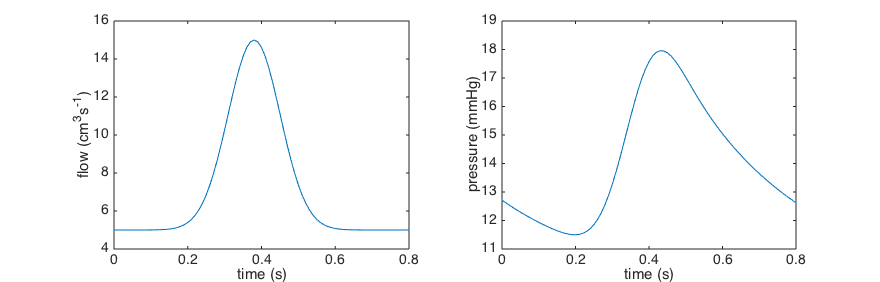
\includegraphics[width=\textwidth]{flowpressureRCR.png}
\end{center}

We get a pressure output different (in magnitude, but similar in shape !) from the one available in Gerbeau's work. However, we would like to test UKF and EnKF on this testcase.



\stepcounter{c}
\setcounter{d}{0}
\setcounter{e}{0}
\setcounter{d}{0}
\setcounter{r}{0}
\paragraph{\arabic{c} - Data assimilation : Kalman filters}

We now wish to find values of $R_1,R_2$ and $C$ matching observation of $p$. Observed $p$ will be simulated by noising the previously computed pressure.


We have to consider the following dynamical system :

\eq{
\left\{
\begin{array}{l}
\displaystyle C\frac d{dt}p+\frac p{R_2}=CR_1\frac d{dt}q+\left(1+\frac{R_1}{R_2}\right)q\\
\displaystyle \frac{dR_1}{dt}=0\\
\displaystyle \frac{dR_2}{dt}=0\\
\displaystyle \frac{dC}{dt}=0
\end{array}
\right.
}

\noindent Its input is $q$ and the state variable is $\mathbf x=(p,R_1,R_2,C)^T$. The measurement is performed through the matrix :

$$H=\left(\begin{array}{cccc}1&0&0&0\end{array}\right)$$

The joint state-parameter estimation giving awful results, we performed successive state-parameter estimation based on Ensemble Kalman Filter.
\end{document}